 \documentclass[11pt,a4paper]{article}
\usepackage[utf8]{inputenc}		% LaTeX, comprend les accents !
\usepackage[T1]{fontenc}
\usepackage{natbib}	
%\usepackage[square,sort&compress,sectionbib]{natbib}		% Doit être chargé avant babel      
\usepackage[frenchb,english]{babel}
\usepackage{lmodern}
\usepackage{amsmath,amssymb, amsthm}
\usepackage{a4wide}
\usepackage[capposition=top]{floatrow}
\usepackage{verbatim}
\usepackage{float}
\usepackage{placeins}
\usepackage{flafter}
\usepackage{longtable}
\usepackage{import}
\usepackage{pdflscape}
\usepackage{rotating}
\usepackage{hhline}
\usepackage{multirow}
\usepackage{booktabs}
\usepackage[pdftex,pdfborder={0 0 0},colorlinks=true,linkcolor=blue,urlcolor=blue,citecolor=blue,bookmarksopen=true]{hyperref}
\usepackage{eurosym}
%\usepackage{breakcites}
\usepackage[autostyle]{csquotes}
%\usepackage{datetime}
\usepackage{natbib}
\usepackage{setspace}
\usepackage{lscape}
\usepackage[usenames]{color}
\usepackage{indentfirst}
\usepackage{url}
\usepackage{enumitem}
\usepackage{multirow}
\usepackage{subcaption}
\usepackage[justification=centering]{caption}
\usepackage{pdfpages}
\bibliographystyle{agsm}



\usepackage{array}

\newcommand{\isEmbedded}{true}

\graphicspath{{Figures/}}


\begin{document}

\selectlanguage{frenchb}
\title{Premières estimations}


\author{}


\maketitle

\section{Sélection de l'échantillon}
On sélectionne les agents qui sont Adjoints Techniques Territoriaux en 2011. On choisit ce corps pour deux raisons : ce corps est le corps le plus peuplé de la FPT et de la FPH et c'est pour ce corps qu'on a la meilleure qualité de donnée. On se limite aux agents étant dans ce corps pour la première année d'observations complètes afin de réduire le nombre de cas pour lesquels il faudra inférer une position sur les grilles l'année précédente. \bigskip

On sélectionne les agents qui ont leur indice brut et leur code grade CIR renseignés en 2011, ce qui permet de les replacer sur une grille.
\begin{center}
	\begin{tabular}{llr}
		\toprule
		{} &                                         Filtre &       Nombre d'agents \\
		\midrule
		0 &                                     Aucun &  367583 \\
		1 &                     Corps des ATT en 2011 &  272413 \\
		2 &                         Génération > 1960 &  258085 \\
		3 &  Code cir nul et état activité après 2010 &  238613 \\
		4 &            IB manquant entre 2007 et 2015 &  197639 \\
		5 &             Rattaché à une grille en 2011 &  187102 \\
		\bottomrule
	\end{tabular}
\end{center}


\section{Statistiques descriptives}
\begin{figure}[H] 
	\caption{Histogrammes des durées minimales passés dans chaque grade du corps ATT}
	\label{transit1} 
	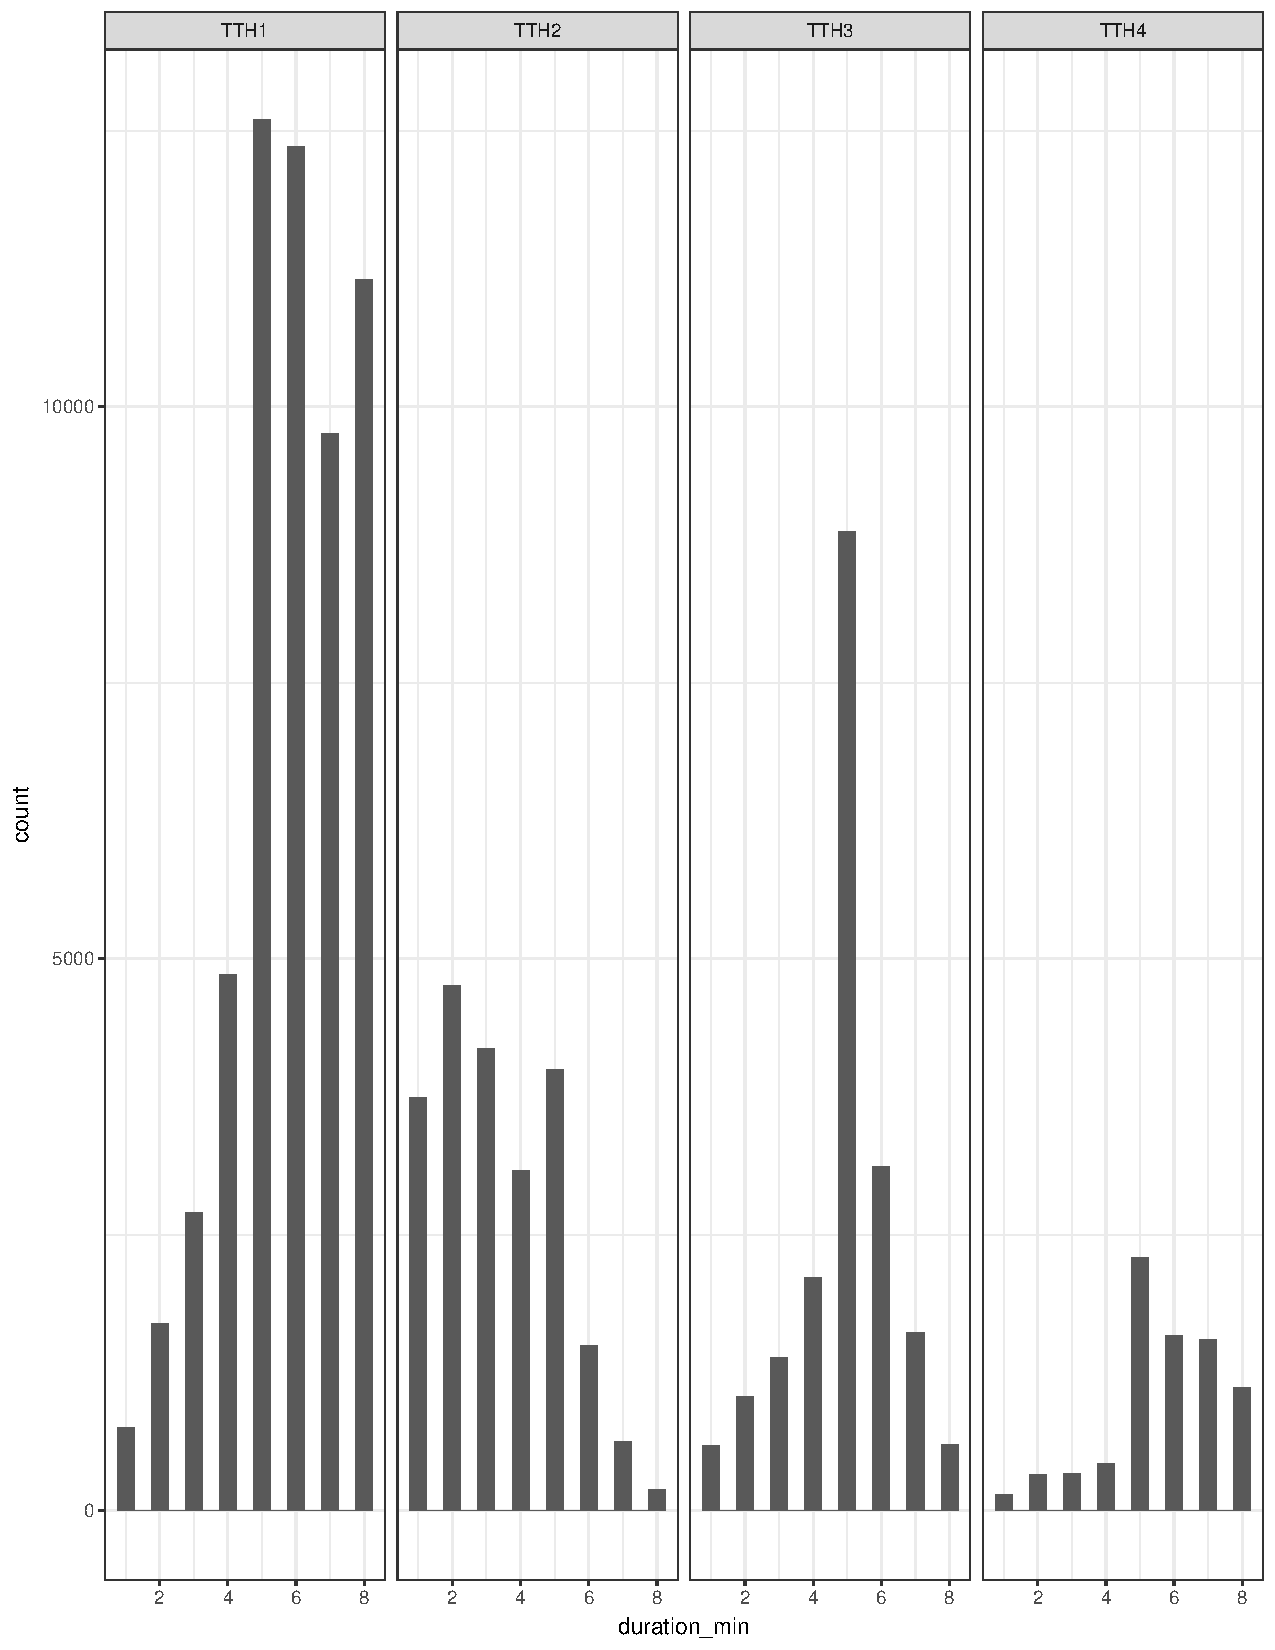
\includegraphics[width = 15cm, height=7cm, keepaspectratio]{hist_duration_min.pdf} 
\end{figure}
\begin{minipage}{15cm}
	\footnotesize
	\textsc{Population:} Agents auxquels on a appliqué les filtres de la section 1, qui sont non censurés à gauche (i.e qui sont pour sûr entrés dans leur grade de 2011 entre 2007 et 2011). 105 057 agents sont représentés. 58 127 durées sont censurées à droite.\\
\end{minipage}

\begin{figure}[H] 
	\caption{Histogrammes des durées maximales passés dans chaque grade du corps ATT}
	\label{transit1} 
	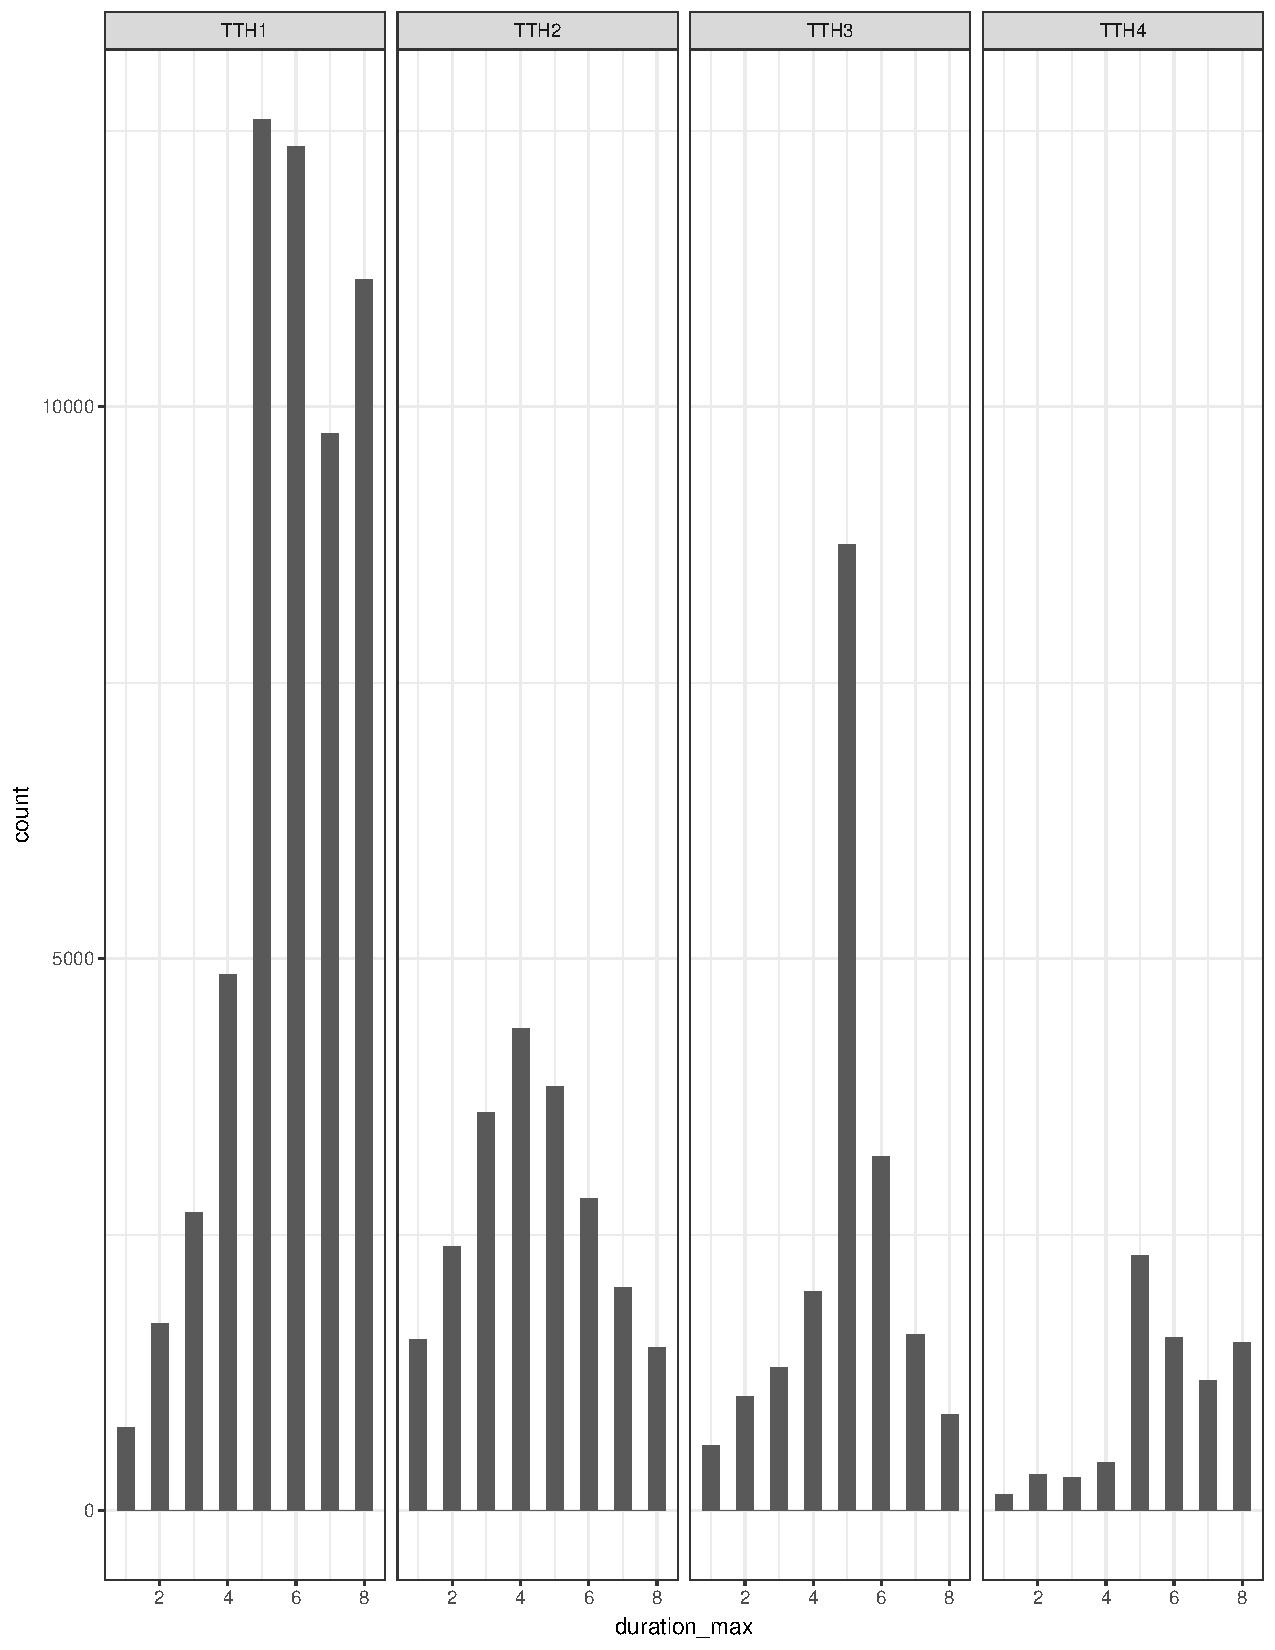
\includegraphics[width = 12cm, height=7cm, keepaspectratio]{hist_duration_max.pdf} 
\end{figure}
\begin{minipage}{15cm}
	\footnotesize
	\textsc{Population:} Agents auxquels on a appliqué les filtres de la section 1, qui sont non censurés à gauche (i.e qui sont pour sûr entrés dans leur grade de 2011 entre 2007 et 2011). 105 057 agents sont représentés. 58 127 durées sont censurées à droite.\\
\end{minipage}

\begin{figure}[H] 
	\caption{Histogramme de la censure à droite par grade}
	\label{transit1} 
	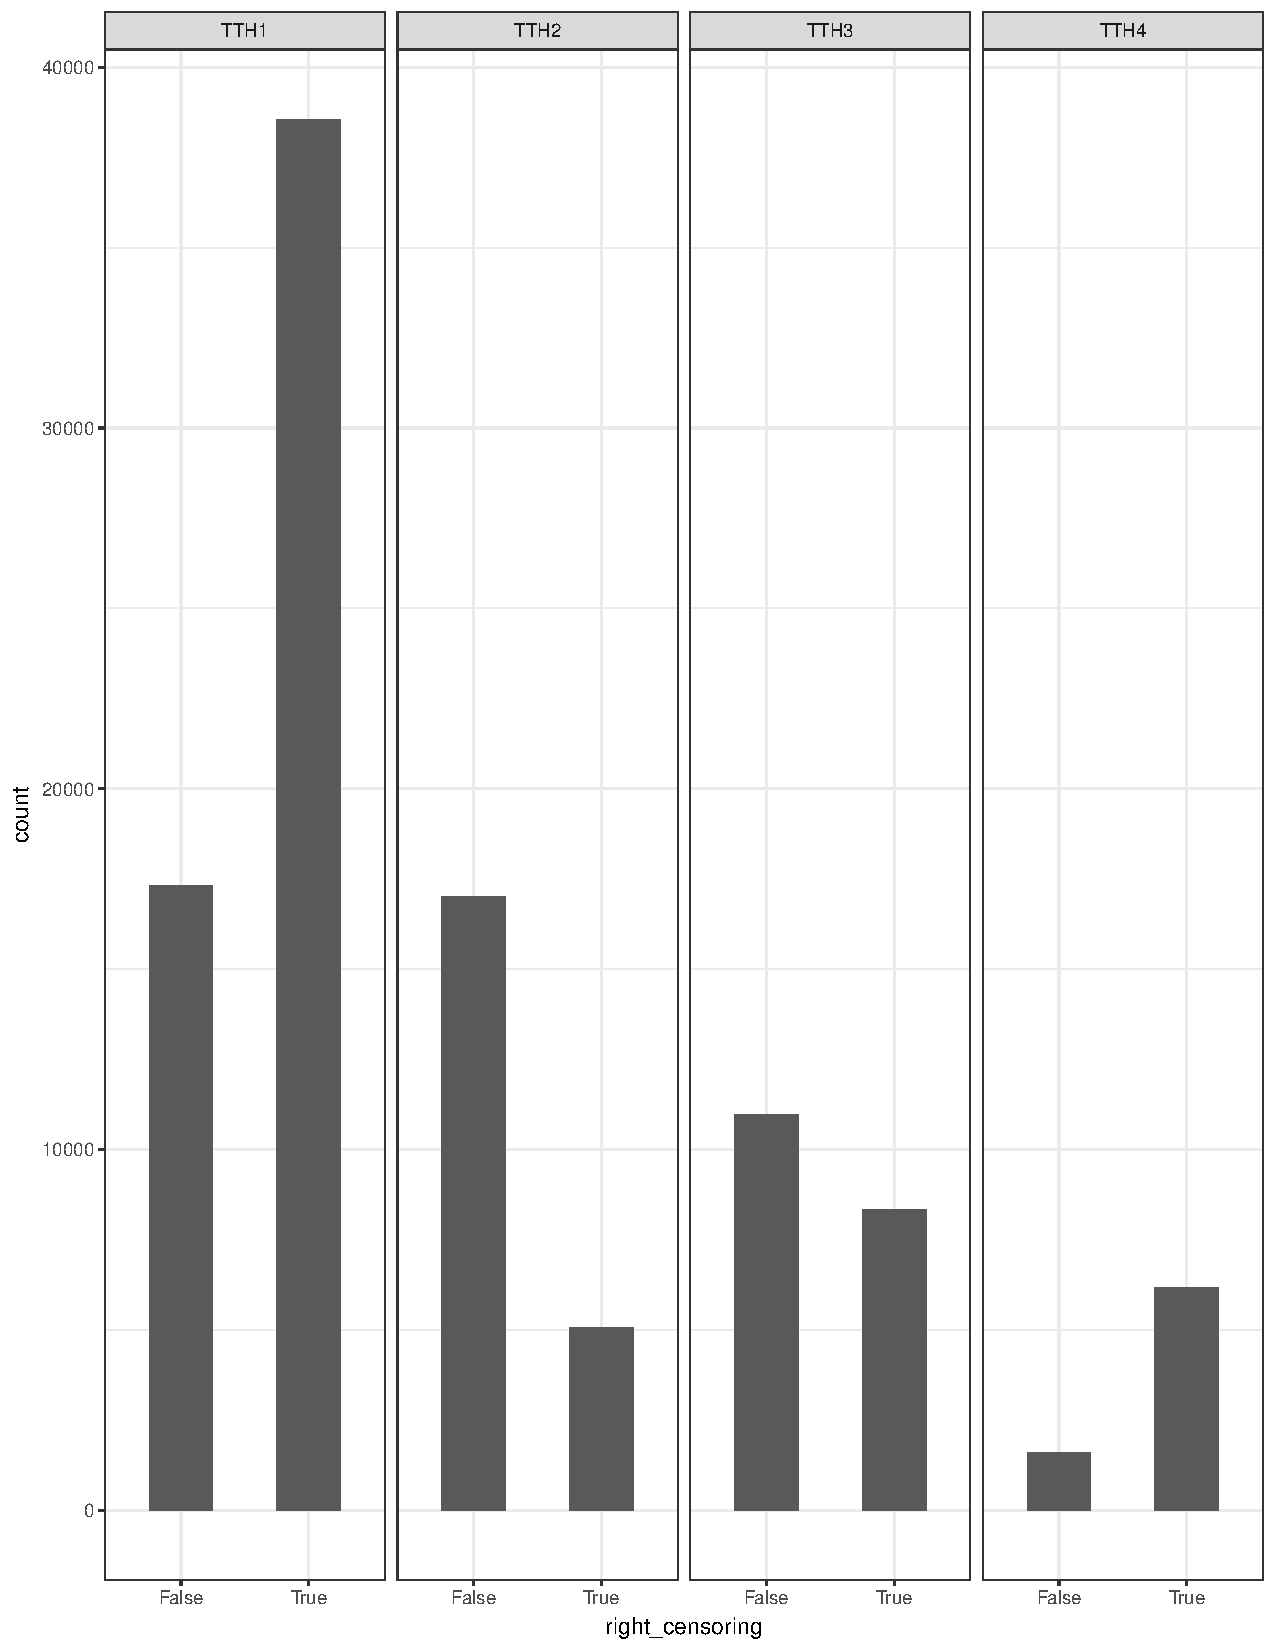
\includegraphics[width = 12cm, height=10cm, keepaspectratio]{right_censoring_par_grade_de_2011.pdf} 
\end{figure}
\begin{minipage}{15cm}
	\footnotesize
	\textsc{Population:} Agents auxquels on a appliqué les filtres de la section 1, qui sont non censurés à gauche (i.e qui sont pour sûr entrés dans leur grade de 2011 entre 2007 et 2011). 105 057 agents sont représentés. 58 127 durées sont censurées à droite.\\
\end{minipage}

\bigskip



\end{document}